\section{Approach Operationalization}
\label{sec:operationalization}
In this section, we propose an operationalization of our approach.
We present the implementation of a compiler which transforms a query into a Java program calling the SWH Graph API.
We first discuss our choice of the Object Constraint Language (OCL)~\cite{DBLP:conf/sfm/CabotG12} to specify the query, then how we manage timestamps.
Finally, we explain how the implemented process generates a executable program from the formers to retrieve SWHIDs of the matching repositories.

\begin{figure*}
    \center 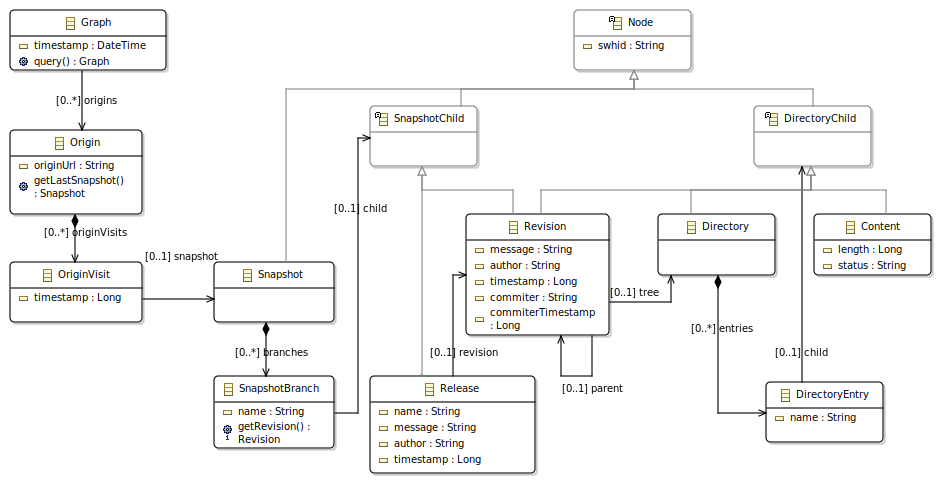
\includegraphics[width=0.8\textwidth]{images/swhModel.png}
    %\vspace{-5 pt}

    \caption{Object Model of the SWH Graph Dataset}
    \vspace{-5 pt}

    \label{fig:swhModel} 

\end{figure*}

\subsection{Dataset Specification}

To formally describe a subset of the repositories included in the SWH Graph Dataset, we rely on a query expressed in a query language.
Several query languages exist which can be used for this purpose.
When selecting a query language, we considered the language expressiveness and the facility to use the language for code generation purpose.

SQL can be used with the relational version of the archive metadata, but as we said previously, this solution is not appropriate to express complex queries due to the graph nature of the archive.
Graph query languages such as \emph{GraphQL}~\cite{DBLP:conf/www/Hartig018} or \emph{Cypher}~\cite{DBLP:conf/sigmod/FrancisGGLLMPRS18} could be used on the compressed version of the graph.
However, we found that GraphQL has some limitations regarding its expressiveness (lack of conditional support, join operation or user defined function) and does not allow transitive closure.
Cypher addresses most of the limitations mentioned for GraphQL, making it a good candidate as our query description language. 
However, the lack of tooling facilitating the creation of generators or an available editor has led us to discard this language. 

OCL (Object Constraint Language) is an object query language allowing to describe constraints on an object-oriented model, which can also be used to express complex queries without side effects.
OCL is widely used in the model-driven engineering community and comes with numerous tools, such as the Eclipse OCL implementation enabling to express constraints on a UML or an Ecore model.
It also provides an editor and facilities for creating generators. 
To be able to express OCL queries on the archive metadata,   
we defined an object-oriented model of the SWH Graph Dataset (Fig.~\ref{fig:swhModel}) representing the different elements considered in the metadata schema. 
The model conforms to the structure of the compressed graph described in~\cite[Chapter 10]{pietri:tel-03515795}.
An instance of this model represents an export of the Software Heritage archive.
The \texttt{Graph} class thus represents a specific version of the Graph Dataset.
It is composed of a list of repositories and a timestamp representing the version of the export. 
The repositories are represented by the \texttt{Origin} class and are identified by their URLs.
Every time a repository is crawled by SWH, the state of the repository is captured by a timestamp and a snapshot as an \textit{OriginVisit}. 
The rest of the model is similar to the Git Merkle DAG. 
Indeed, a \texttt{Snapshot} is composed of a list of \texttt{SnapshotBranch}es pointing to a \texttt{Revision} (equivalent of a Git commit) or a \texttt{Release} (equivalent of a Git tag). 
Finally, each \texttt{Revision} is composed of a file tree and a reference to the previous \texttt{Revision}. 
The \texttt{Snapshot, Release, Revision, Directory} and \texttt{Content} classes inherit from the Node interface and are identified by SoftWare Heritage persistent IDentifiers (SWHIDs) which are guaranteed to remain resolvable over time.\footnote{\url{https://docs.softwareheritage.org/devel/swh-model/persistent-identifiers.html}} The SWHID also enables integrity check of an entire snapshot since it contains the SHA1 hash of the referenced object.


\begin{figure}[ht]
\begin{lstlisting}
import swhModel : 'platform:/resource/.../swhModel.ecore'
package swhModel
context Graph
def : query():Set(Origin) = origins->select(
	 getLastSnapshot().branches->exists(
	 	(name='refs/heads/master' or name='refs/heads/main')
		and
		/*The branch contains at least 1000 revisions */
		getRevision()->closure(parent)-> size() >1000
		and
		/*The root revision have been created since 2015 */
		getRevision().getRootRevision().commiterTimestamp>1420066800
		and
		/*The branch contains a file 'AndroidManifest.xml'*/
		getRevision().tree.entries->closure(entry:DirectoryEntry |
				if entry.child.oclIsKindOf(Directory) then
					entry.child.oclAsType(Directory)
                        .entries.oclAsSet()
				else 
					entry.oclAsSet()
				endif	
		)->exists(e:DirectoryEntry | e.name='AndroidManifest.xml')))
context Revision
 def : getRootRevision() : Revision =
	  if parent = null then self
    else parent.getRootRevision() endif
endpackage

\end{lstlisting}
%\vspace{-1em}
\caption{The running query expressed in an OCL expression}
\label{fig:OCL_query}
\end{figure}
 
OCL allows to define methods without side effects over the classes of a given model, hence enabling to express queries on this model.
Figure~\ref{fig:OCL_query} presents an OCL query corresponding to our illustrative example about Android applications (Section~\ref{sec:motivations}).
The first line of the OCL file indicates the model: in our case, \texttt{swhModel.ecore} is the model presented in Fig.~\ref{fig:swhModel}.
We define a method named \textit{query} (line 4) which returns a set of \texttt{Origins} (repositories) when applied to an instance of the class \texttt{Graph} (\texttt{context Graph}, line 3).
In other words, this method takes a version of the SWH archive and selects repositories matching the filters defined in the query (lines 4 to 24).
We can see in line 5 that we select the origins whose last snapshot contains at least a branch matching the following conditions:
  \begin{itemize}
      \item Line 6: The branch name must be ``main'' or ``master''.
      \item Line 9: The branch must contain at least 1000 revisions, we used the closure operation on the last revision of the branch to flatten the parent revision relation. 
      \item Line 12: The root revision must have been created after 2015. We define the ``\texttt{getRootRevision()}'' operation in the \texttt{Revision} context (lines 25-31) to retrieve the first revision of a branch.
      \item Lines 15-22: The revision must contain an entry named \\``\texttt{AndroidManifest.xml}''. The file tree of the revision is flattened into a set of \textit{DirectroryEntry} with a closure operation.
  \end{itemize}

\subsection{Timestamp Management}

The SWH archive is continuously evolving over time by crawling snapshots of repositories and updating the current archive state. The model of Fig.~\ref{fig:swhModel} contains two types of timestamps. The timestamp in \texttt{OriginVisit} defines the time where the snapshot of a given repository was taken.
The timestamp in \texttt{Graph} indicates a frozen version of the Graph Dataset which contains all the \textit{OriginVisit}s taken before this timestamp. 

Both timestamps allow us to fix the state of the archive on which the query will be executed and ensure that the query output will be reproducible for a given timestamp.  
Since the SWH archive is immutable, it is theoretically possible to filter a given export to retrieve the state of a previous export and execute a \textit{query} on it. 
In other words, if we run a query \texttt{q} on an export realized at a time $t$, re-running the same query \texttt{q} on an export done at a time $t+m$ while discarding all the \textit{OriginVisit}s  added after $t$ should produce the same selection.

\subsection{Repository Selection}

To automate the selection of the repositories from the SWH archive that match the filters expressed in the OCL query, we implemented a compiler translating the constraints of the query in an optimized Java program which uses the SWH-Graph API to perform filtering operations on the SWH Graph Dataset. 

We first wrapped the SWH-Graph API to conform to the object-oriented model of Fig~\ref{fig:swhModel}.
Indeed, the SWH-Graph API is not fully object-oriented, and relies on static methods to retrieve node properties  to improve its efficiency (i.e., avoiding object creation). 
Wrapping this API to the same OO model highly facilitates the translation of the OCL query in Java code.

The compiler relies on a generator taking as input an OCL query.
First, it uses Eclipse OCL PIVOT, which provides an Xtext grammar of OCL, to build the Abstract Syntax Tree (AST) of the query.
The obtained AST is then traversed to generate the corresponding Java code.
For this, we specify in the generator one generation method for each type of nodes of the AST, defining the Java code to be produced if this type of node is encountered during the traversal.
For instance when the \textit{exists} OCL operation is used in the query, it will trigger the generation method of the \textit{IteratorExp} node type and produce Java code using \textit{stream().anyMatch()}.
Visiting the entire AST thus produces the corresponding executable Java code calling the SWH-Graph API to select repositories.

Executing this code outputs the set of SWHIDs referring to \textit{Origin}s (repositories) matching the constraints expressed in the initial query. 
Then, this set of origin IDs is possibly used to extract the sub-graph of the SWH Graph Dataset restricted to the provided origins, in both column based or compress format. 

The source code of the compiler is available on the replication package associated to this paper.\footnote{https://doi.org/10.5281/zenodo.7989955}